\documentclass[../../AdvancementSummary.tex]{subfiles}

\begin{document}



%%%%%%%%%%%%%%%%%%%%%%%%%%%%%%%%%%%%%%%%%%%%%%%%%%%
\section{Local structuring of disordered signaling proteins gives rise to cooperativity and sequential binding}
\label{sec:LocalStruct}
%%%%%%%%%%%%%%%%%%%%%%%%%%%%%%%%%%%%%%%%%%%%%%%%%%%


\subsection{Introduction}

%\hl{Intrinsically disordered proteins sterically occlude ligands by transiently sequestering the binding site.} 

There is evidence that indicates some IDPs undergo a disordered-to-ordered transition upon post-translational modification, i.e. phosphorylation. For example, phosphorylation of PAGE4 restricts the number of conformations it may explore, increasing rigidity of the backbone \cite{He2015}. Similarly, a segment of the protein Tau, has been shown to have increased persistence length upon multiple phosphorylation \cite{Chin2016}. Post-translational modifications may also cause a conformational change, altering the availability of the binding site. The neural protein 4E-BP2 undergoes multisite phosphorylation which leads to a disorder-to-order transition, forming $\beta$ sheets which hide the eIF4E binding site \cite{Bah2015}. 

Initial models of the TCR $\zeta$ chain indicate large enhancements of the phosphorylation rate can occur assuming a complete switch from disorder to order upon initial phosphorylation. Binding to a fully structured protein compared to a disordered protein can be ~100 fold easier, depending on the persistence length and ligand size \cite{Mukhopadhyay2016}.

%From our simple model of a disordered protein, we may answer some basic questions. What is the probability that a ligand will be able to bind a specific site on a cytosolic disordered protein?  How does this probability change when the protein is anchored to the membrane?  How do these probabilities change with the contour length of the protein, size of the ligand, and where the binding site is located along the length of the protein?

We are interested in how cooperative effects may arise in reactions with a disordered protein. One model we explore is disorder-to-order transitions as a result of post-translational modifications. With regards to our case study, CD3$\zeta$, we assume that each phosphorylation event causes a fraction of the chain to undergo a disorder-to-order transition. Partial structuring will reduce the number of conformations available to the protein. We predict this will increase the number of conformations where a ligand may access its binding site due to a forced linearization of part of the chain. We investigate how this local structuring phenomenon would impact subsequent phosphorylations by Lck along TCR CD3$\zeta$. Specifically, we want to know if local structuring of a disordered protein upon multi-site phosphorylation can induce enhancement of subsequent binding events.

%%%%%%%%%%%%%%%%%%%%%%%%%%%%%%%%%%%%%%%%%%%%%%%%%%%%%%%%%%%%%%%%%%%%%%%%%%%%%%%%%%%%%%%%%%%%%%%%%%%%%
%%%%%%%%%%%%%%%%%%%%%%%%%%%%%%%%%%%%%%%%%%%%%%%%%%%%%%%%%%%%%%%%%%%%%%%%%%%%%%%%%%%%%%%%%%%%%%%%%%%%%
\subsection{Model and Methods}

We model the TCR CD3$\zeta$ chain as a freely jointed chain, where each amino acid is represented as a segment as described in Sec. \ref{sec:ModelDev}. The unbound ligand is simulated as an idealized ghost sphere located tangential to a single segment. We calculate quasi-equilibrium statistics for the FJC and unbound ligand in both free-space and half-space. For the CD3$\zeta$ chain, we simulate only the cytoplasmic region by an FJC with 113 segments. In our simulation, all lengths are normalized by the Kuhn length, so each rod has length 1 and the radius of the ligand is also measured in Kuhn lengths. We consider a spherical estimate for the kinase Lck, with a radius of 2.1\nm (7 Kuhn lengths) as calculated in Sec. \ref{sec:ModelDevsubsec:TCR}.

We calculate how often a ligand is able to bind to an oriented sphere tangentially attached to the polymer, where `able to bind' refers to the specified sphere being empty of both other polymer segments and the surface, if present. 

We include local structuring as a limitation on which joints of the freely jointed chain are allowed to rotate. For each modified residue, some number of joints are `frozen' in a straight conformation (Fig. \ref{fig: StiffeningCartoon}). The section of frozen segments acts as a single long segment, still rotating when other neighboring segments rotate. This method of local structuring leaves the original binding site in a primarily available configuration, however, we are interested in how it impacts the neighboring modification targets (i.e. tyrosines to be phosphorylated). We explore how the total number of structured residues per modification impacts the result. 

\begin{figure}[H]
\begin{center}
    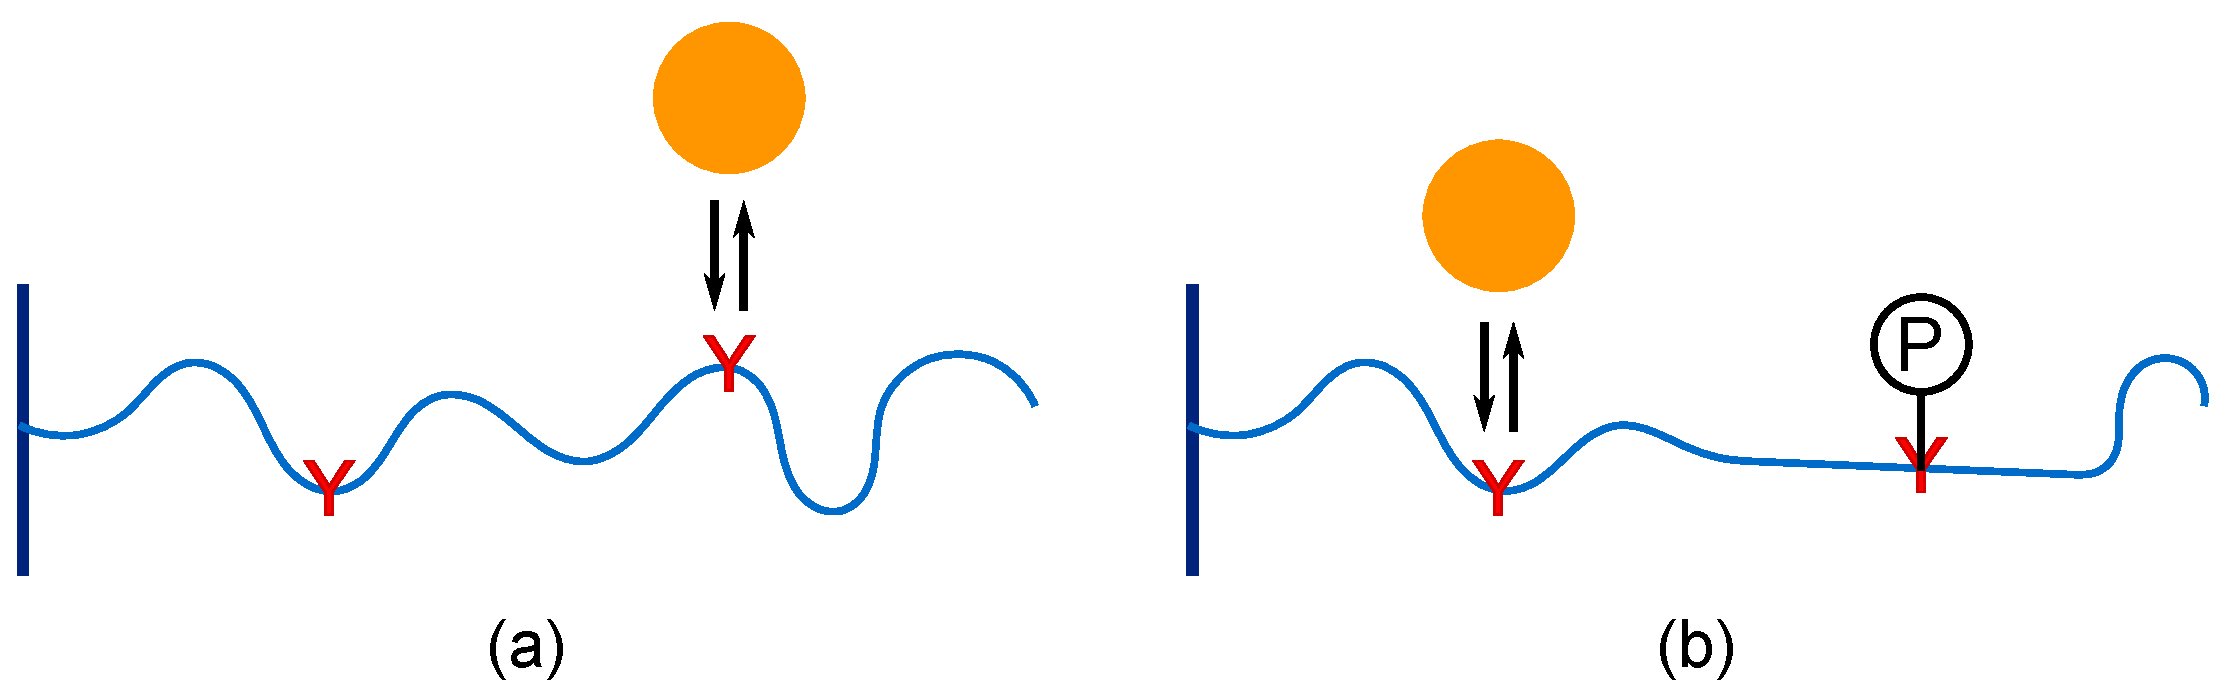
\includegraphics[width=0.8\linewidth]{ResultsFigures/StiffeningDiagram/StiffeningDiagram.eps}
    \caption{Cartoon of partial stiffening model. Entirely floppy FJC prior to modification (a) transitions to partially rigid chain after modification (b). \label{fig: StiffeningCartoon}}
    \end{center}
\end{figure}

For TCR CD3$\zeta$, phosphorylation events are modeled as creating local structure as described above. Similarly, we model dephosphorylation as `unfreezing' nearby segments. Since we will eventually model reversible phosphorylation, we consider the case where the initial polymer state is only as stiff as it would be from the local stiffening by full phosphorylation. For example, if phosphorylation would locally structure the nearest eleven segments, then the fully phosphorylated form of CD3$\zeta$ would have 66 residues frozen. We use this as the initial state for dephosphorylation. Each dephosphorylation would unstructure 11 of the initial 66 frozen residues. For simplicity, we assume the phosphatase is the same size as the ligand Lck.


%%%%%%%%%%%%%%%%%%%%%%%%%%%%%%%%%%%%%%%%%%%%%%%%%%%%%%%%%%%%%%%%%%%%%%%%%%%%%%%%%%%%%%%%%%%%%%%%%%%%%
%%%%%%%%%%%%%%%%%%%%%%%%%%%%%%%%%%%%%%%%%%%%%%%%%%%%%%%%%%%%%%%%%%%%%%%%%%%%%%%%%%%%%%%%%%%%%%%%%%%%%
\subsection{Results}

\subsubsection{Surface presence influences polymer configuration}
%\hl{ don't really like 'due to entropic forces....?}
We first explore how a freely-jointed chain is affected by the presence of a surface or membrane. Generally, FJCs are most likely to be in a `hairball' conformation due to entropic forces. When we compare the end-to-end distances of a FJC in free space to a FJC in half space, we find a shift in the distribution. The half-space polymer tends to have a larger end-to-end distance than the free-space polymer (Fig. \ref{fig: ReeHalfVSFree}). In half space, the polymer has fewer conformations it can take on since it can only occupy half of the region. This prevents many more `hairball' conformations than it prevents straightened conformations. Overall, the presence of a membrane straightens the polymer. 

\begin{figure}[H]
	\begin{center}
		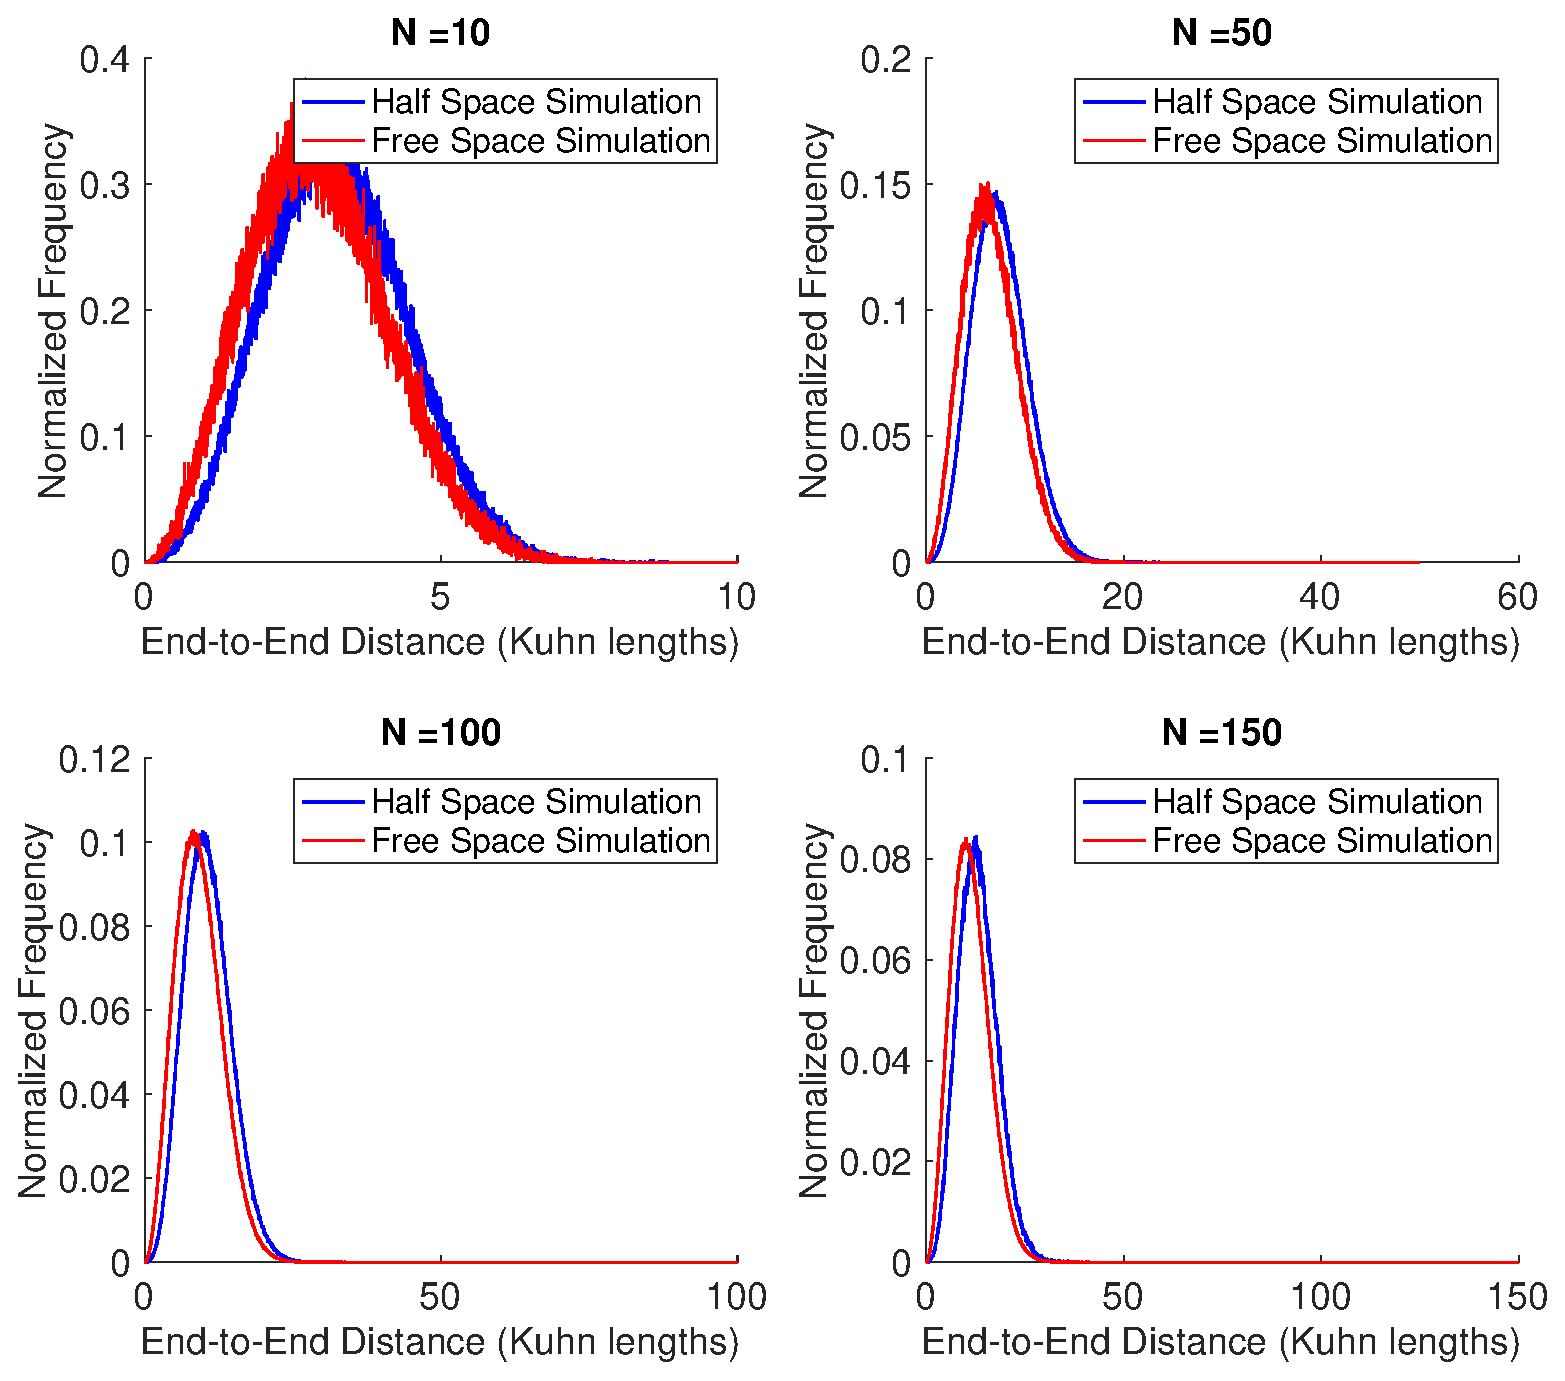
\includegraphics[width=0.8\linewidth]{ResultsFigures/General/ReeDistributionHalfVSFreeSim.eps}
		\caption{Distributions of polymer end-to-end distance in free space and half space for various polymer lengths (N). For each length, the end-to-end distance of the polymer in half-space is overall straighter than in free space.\label{fig: ReeHalfVSFree}}
	\end{center}
\end{figure}

\subsubsection{Disorder inhibits ligand binding}

We calculate how often a ligand may bind to a FJC, under varying characteristics for the FJC. We can see that in free space, the ligand is more occluded when there are more rods and/or the ligand is larger, for a specific binding site (Fig. \ref{fig: OcclusionVSNVSR}). These are both intuitive results. A longer chain creates more conformations where any location on the chain will be occluded by other segments. A shorter or less flexible chain will not be able to bend enough to bury a binding site. A larger ligand will require more space near the binding site to be open, which is naturally less likely.
We also find that the binding site location impacts the occlusion probability. A binding site in the middle of the polymer will also be less available to ligand binding since it is more likely sheltered by the rest of the `hairball' polymer. 

We compare how FJC parameters influence binding in free-space to binding in half-space. The membrane increases the likelihood of straighter conformations, which would be likely to increase the binding probability. However, the membrane itself may also occlude the ligand since we include an orientation of the binding site in our simulation. Therefore if the binding site is oriented down towards the membrane, then even if the polymer is not occluding the ligand, the membrane still might. When we include a hard plane membrane in our simulation, we see that the presence of a membrane generally decreases the probability of ligand binding. When the ligand is small enough, the difference in binding probabilities between free space and half space binding is minimal (Fig. \ref{fig: OcclusionVSNVSR}).

\begin{figure}[H]
\begin{center}
\begin{subfigure}{0.4\linewidth}
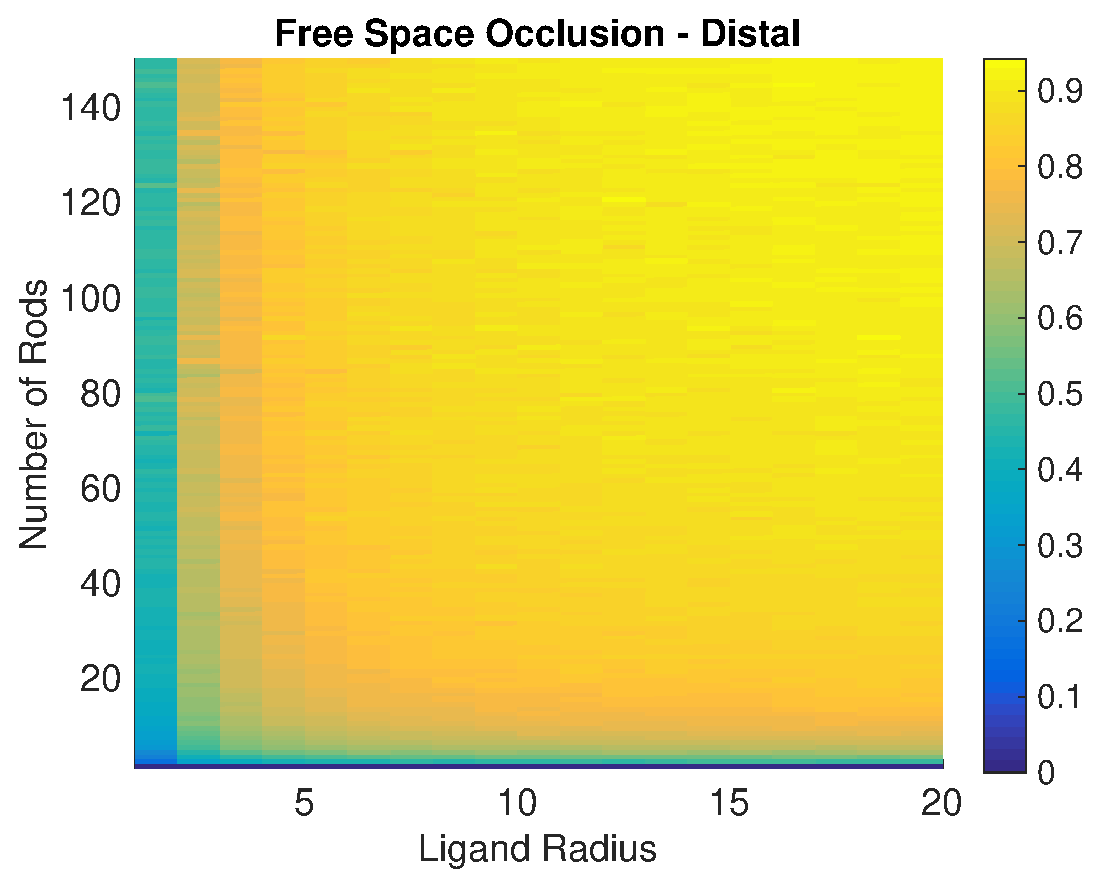
\includegraphics[width=\linewidth]{ResultsFigures/General/OcclusionVSNVSRFree.eps}
\caption{}
\end{subfigure}
\begin{subfigure}{0.4\linewidth}
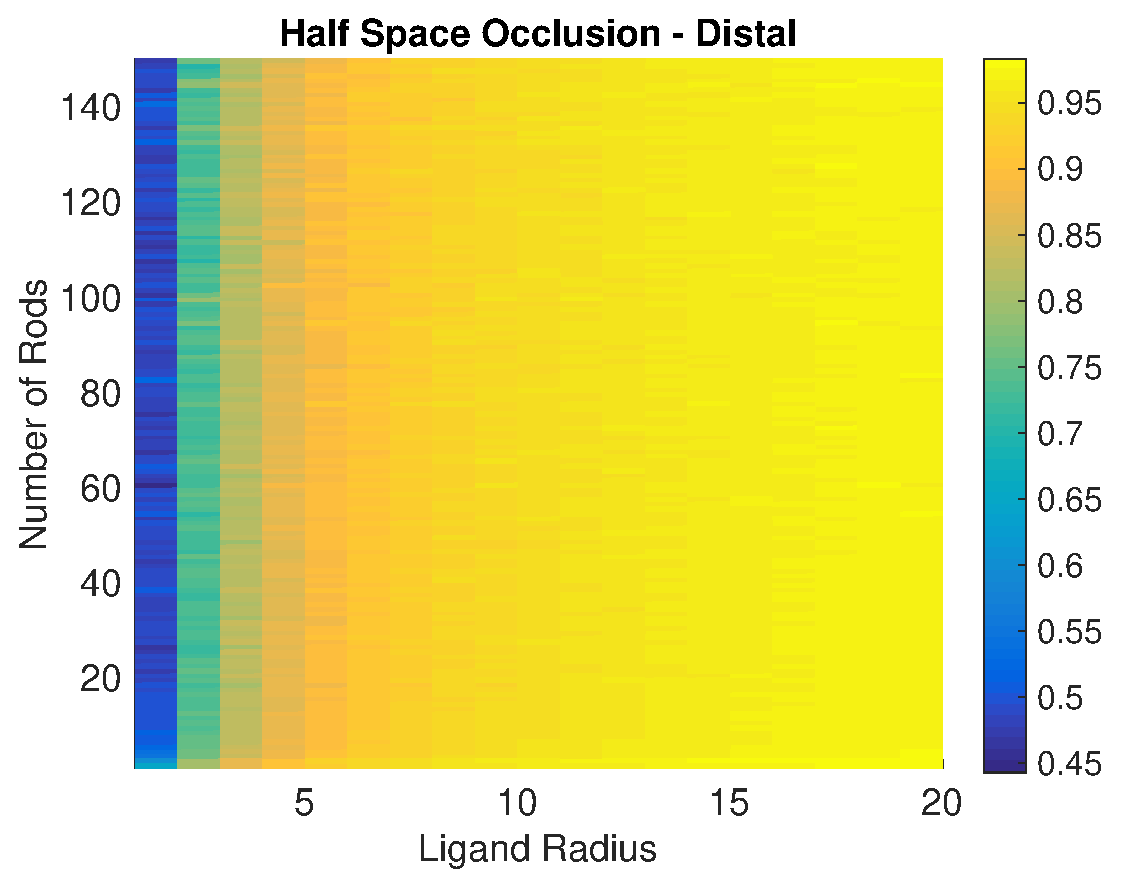
\includegraphics[width=\linewidth]{ResultsFigures/General/OcclusionVSNVSRHalf.eps}
\caption{}
\end{subfigure}
\begin{subfigure}{0.4\linewidth}
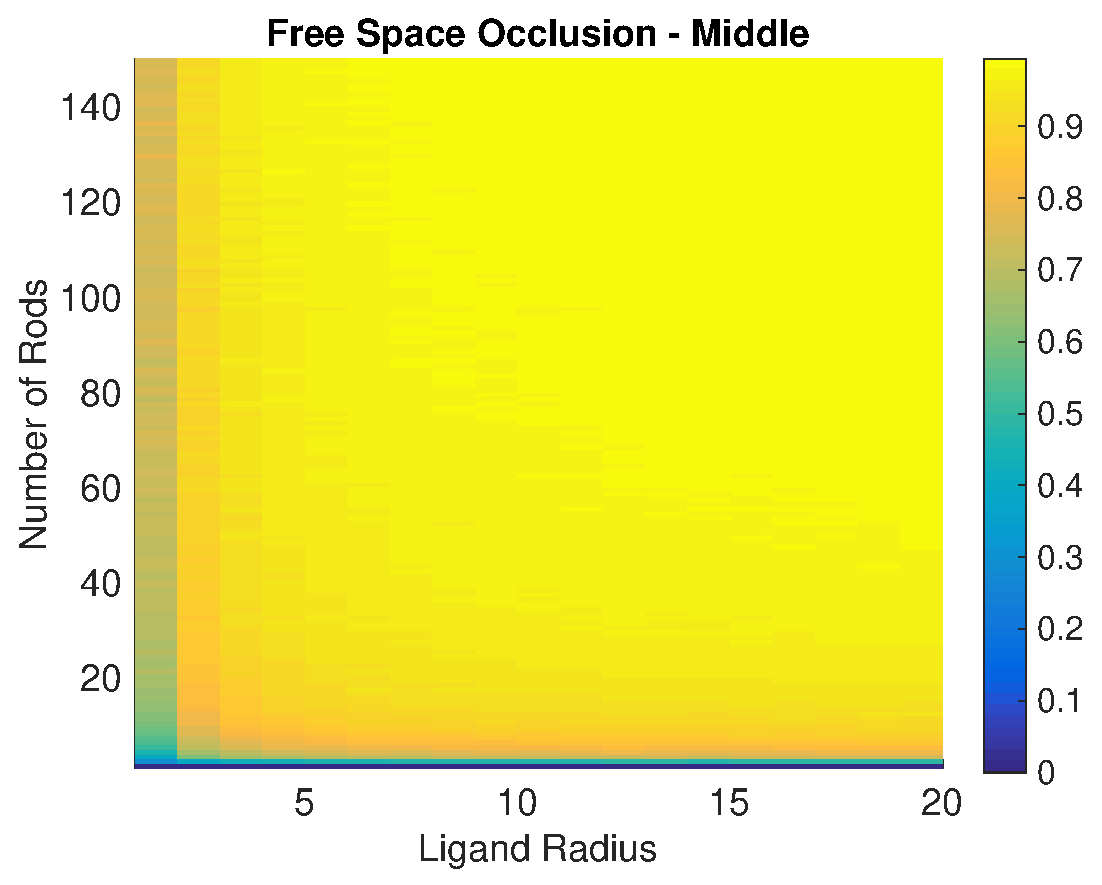
\includegraphics[width=\linewidth]{ResultsFigures/General/OcclusionVSNVSRFreeMid.eps}
\caption{}
\end{subfigure}
\begin{subfigure}{0.4\linewidth}
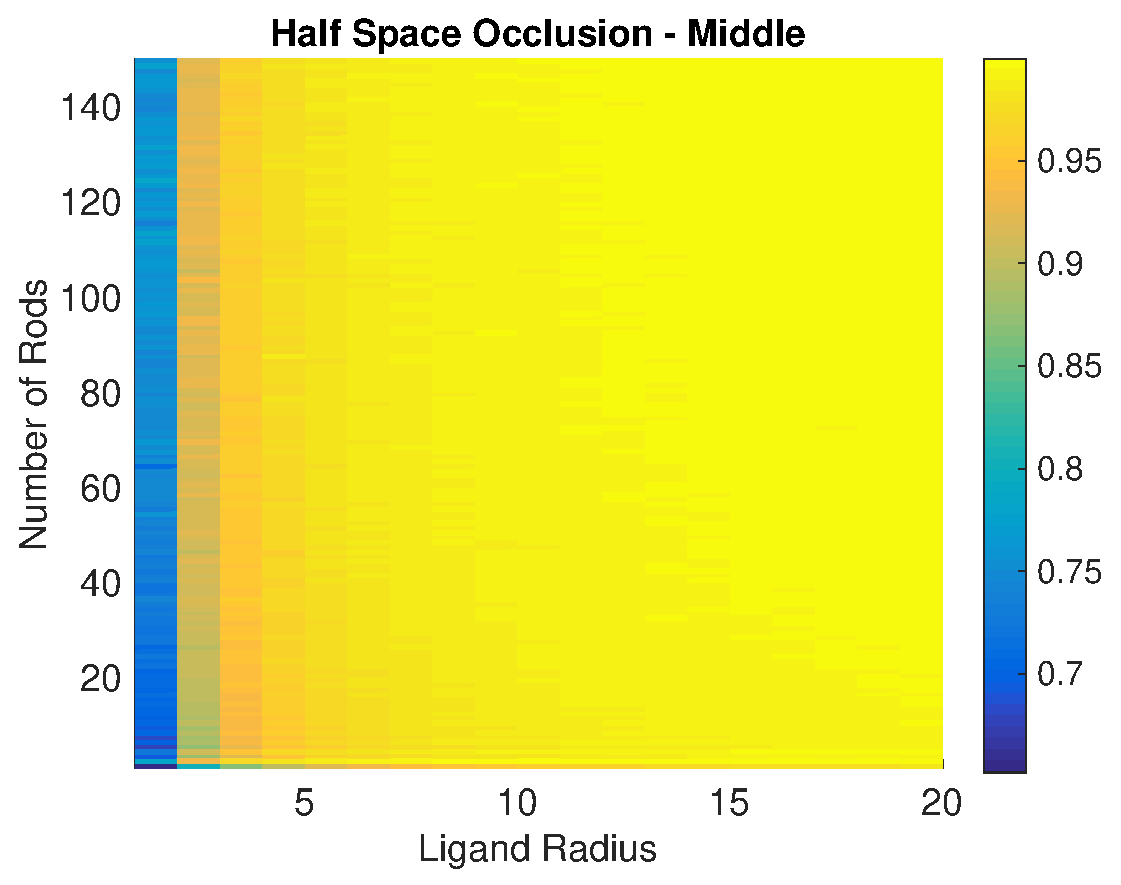
\includegraphics[width=\linewidth]{ResultsFigures/General/OcclusionVSNVSRHalfMid.eps}
\caption{}
\end{subfigure}
\caption{Probability of occluding a ligand of variable radius from a polymer of variable contour length when the binding site is at the distal end or middle of the chain in free space or half space. (a) Free space polymer with binding site at distal end. (b) Half space polymer with binding site at distal end. (c) Free space polymer with binding site in the middle. (d) Half space polymer with binding site in the middle.\label{fig: OcclusionVSNVSR}}
\end{center}
\end{figure}


\subsubsection{Occlusion Probability of End Site VS Analytical Result}

We consider analytical solutions to the simplest case, where the ligand is attempting to bind at the end of the freely-jointed chain in free-space. The probability that a random walk over time 0 to $\delta N$, beginning at the edge of a sphere of radius, $R$, will cross into the sphere at any time is analogous to the probability the ligand is occluded by the freely jointed chain with $N$ segments and Kuhn length $\delta$. In order to solve this analytically, we must assume the random walk begins $\epsilon$ away from the sphere or it will always count as occluded. Then we may formulate as follows for the probability of survival, $p(\vec{x},t)$ when the random walk begins at a starting point, $r=R+\epsilon$:

\begin{equation}\label{eq: diffusion}
	\begin{cases}
		\frac{\partial p}{\partial t} = D \nabla^2 p, \hspace{2cm} p=0 \hspace{3mm}\text{at}\hspace{3mm} r=R\\
		p(\vec{x},0) = \delta(\vec{x}-(R+\epsilon))\\
	\end{cases}
\end{equation}

For an approximation, we consider the solution when $N\rightarrow \infty$.

 \begin{equation}\label{eq: analytic}
  	\begin{cases}
 	q(r)=\mathds{P}(\text{not hit sphere}|x(0)=r) \\
 	0=\frac{2}{r}q'(r)+q''(r) \\
 	q(R) = 0 \\
 	q(r) \rightarrow 1 \hspace{3mm}\text{as}\hspace{3mm} r \rightarrow \infty \\
 	\end{cases}
 \end{equation}

 We assume $\epsilon = 1$ Kuhn length and R measured in Kuhn lengths:

 \begin{align*}\label{eq: analyticSolution}
q(r) &= 1-\frac{R}{r}\\
q(r) &= 1-\frac{R}{R+1} \\
 \end{align*}
 
 We see that when we compare our simulated binding probability to the analytic solution, we get good agreement. This tells us both our code is working as desired and that N=100 is approximately $N \rightarrow \infty$.

 \begin{figure}[H]
 \begin{center}
 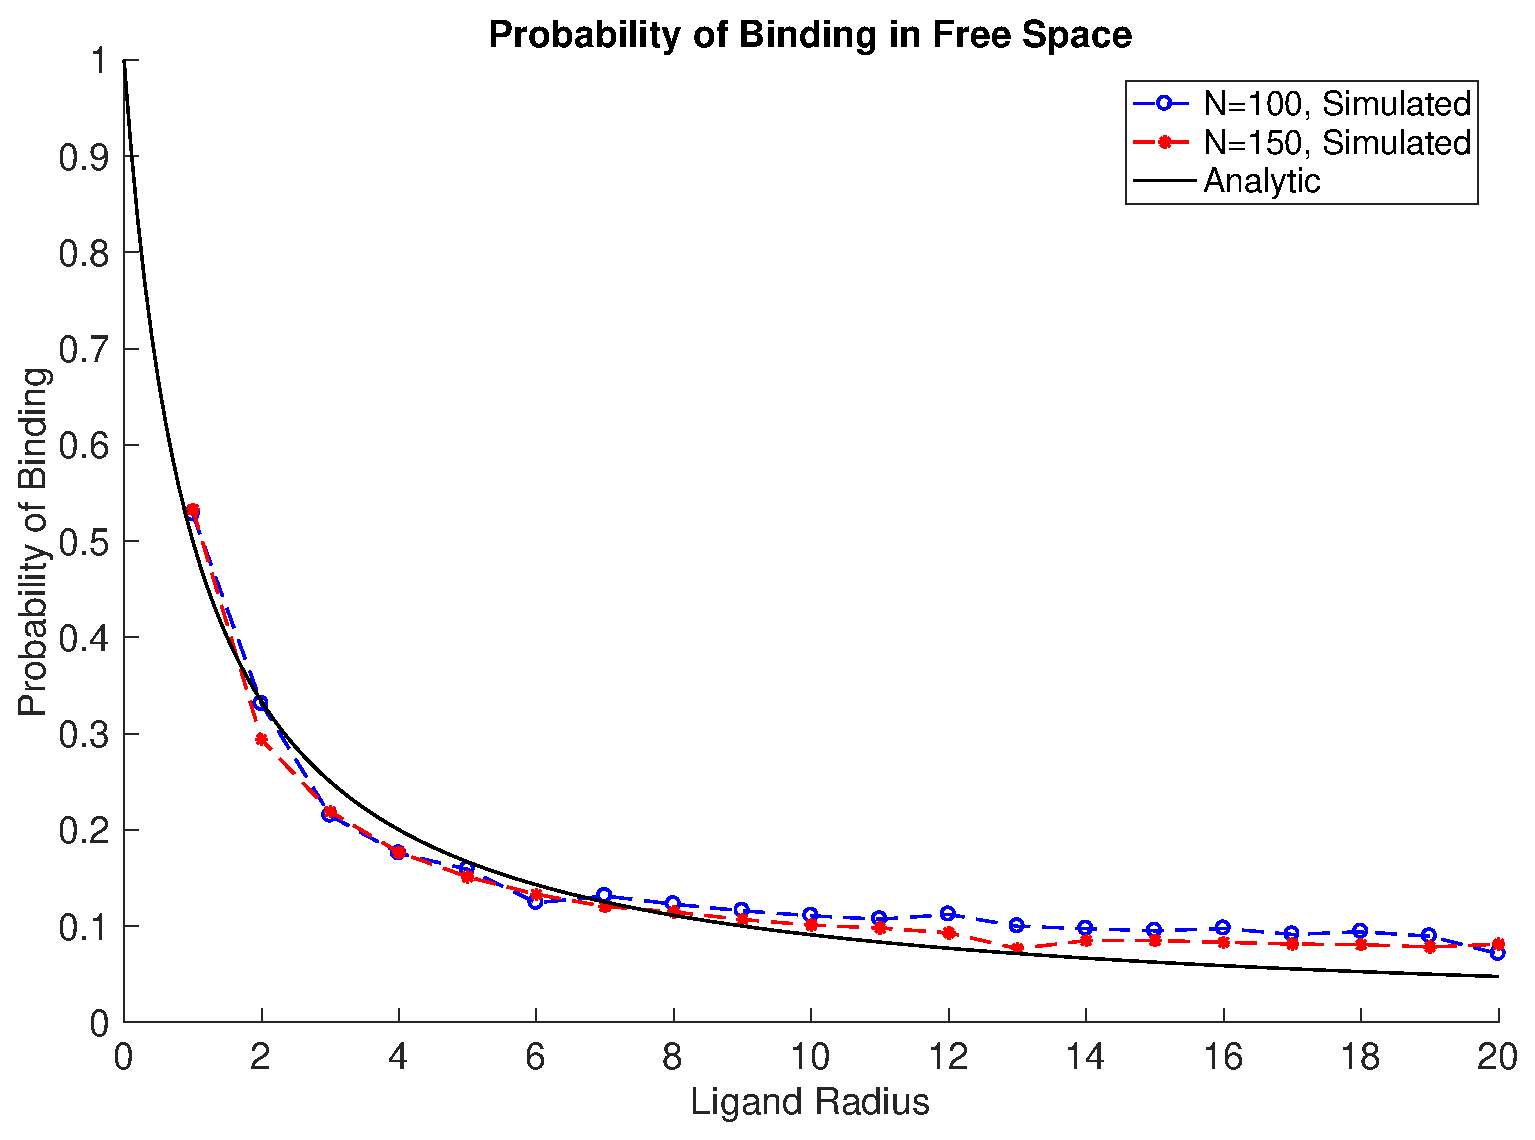
\includegraphics[width=0.7\linewidth]{ResultsFigures/General/Analytic/BindingVSAnalyticN100N150.eps}
 \end{center}
  \caption{Analytic solution (black, solid) compared to occlusion for free-space polymer of 100 Kuhn lengths (blue) and 150 Kuhn lengths (red) for ligands of radius, $R$ Kuhn lengths. \label{fig: AnalyticBinding}}
 \end{figure}



\subsubsection{Cooperativity may arise from local structuring in intrinsically disordered proteins}

We now simulate the kinase Lck binding to the CD3$\zeta$ chain, assuming that each phosphorylation event will create a disorder-to-order transition. If we assume that phosphorylation of tyrosines on the CD3$\zeta$ chain induces local structuring, then neighboring tyrosines will feel a reduction of entropic occlusion. This will cause them to be more available to binding by a ligand. The magnitude of this effect will vary based on how much structuring occurs, e.g. if it affects the nearest two residues or the nearest ten residues. 

We see from these simulations that the average binding rate of a ligand to the unphosphorylated tyrosines increases as the number of phosphorylated tyrosines (and therefore the number of structured residues) increases. From the first to the sixth phosphorylation event, there is a 3-10 fold increase in the average binding rate for moderate (1/12 of chain length) to severe (1/6 of chain length) local stiffening per phosphorylation (Fig. \ref{fig: StiffeningMemOnCoop}).

%\hl{We have 10 fold change. Where does Omer's 100 fold change come in?}

\begin{figure}[H]
	\begin{center}
		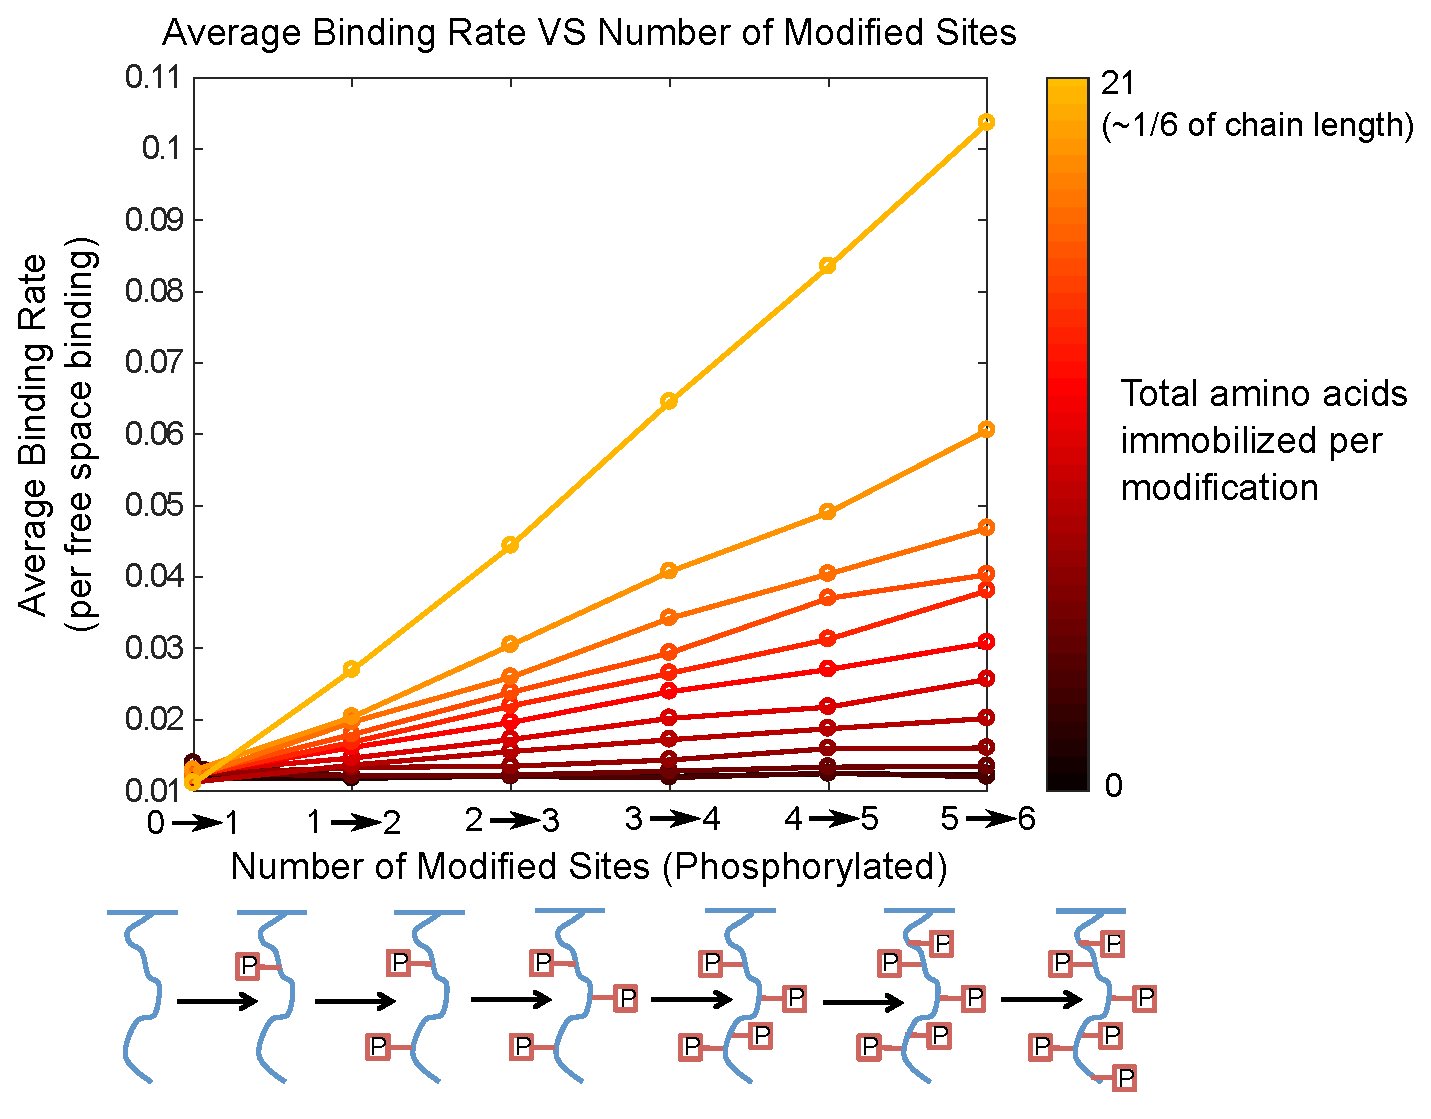
\includegraphics[width=0.8\linewidth]{ResultsFigures/CD3ZetaStiffeningMembraneOn/AvgBindVSTotalPhosColorMapLabeled.eps}
		\caption{(Above) Simulated average binding rates of Lck to CD3$\zeta$ for different levels of phosphorylation given a specified degree of local structuring (none $\rightarrow$ black, low $\rightarrow$ red, high $\rightarrow$ orange). (Below) Cartoon representing a possible phosphorylation state series of CD3$\zeta$. \label{fig: StiffeningMemOnCoop}}
	\end{center}
\end{figure}


\subsubsection{Sequential binding naturally arises from polymer characteristics}

We hypothesized that without any modifications due to binding, then with only the presence of a membrane, we would see preferential binding in an outwards to inwards (6-5-4-3-2-1) manner. In our model system, that is to say we expected the tyrosine furthest from the membrane to be phosphorylated first and the tyrosine closest to the membrane to be phosphorylated last. We surmised this from the idea that tyrosines too close to the membrane would see extra kinase inhibition from membrane occlusion, whereas the tail of the disordered protein would not experience this same effect. 

When considering the partial stiffening model, we predict that this effect would be enhanced. In an unphosphorylated state, if the tyrosine furthest from the membrane is most likely to be bound, then partial stiffening would give increased preference to the next furthest from the membrane (here called the fifth tyrosine) as the second to be phosphorylated. This comes from the reduction of total configurations available to the protein. Since the stiffening would occur around the sixth tyrosine, the nearest unphosphorylated tyrosine would be the most affected. The segment of polymer near the fifth tyrosine would have fewer available conformations and therefore proportionately fewer would be occluding the fifth tyrosine.

We obtained relative probabilities of binding for each tyrosine along the chain at each phosphorylation state. With this information, we are able to explore whether or not there is a dominant sequence of phosphorylation events. We ran a Gillespie algorithm with six events, one for each phosphorylation. From each run, we record which sequence or `path' of phosphorylation. When we compile the path frequency data, we find that the first phosphorylation event is dominant. That is to say, any path beginning by phosphorylating the membrane distal tyrosine (6th tyrosine), will occur more often than any path beginning with the membrane proximal tyrosine. 

For simplicity, we show only the paths membrane proximal to membrane distal (123456) and distal to proximal (654321) (Fig. \ref{fig: StiffeningSeqBind}). We see that when a membrane is present, the probability of phosphorylating distal to proximal is much higher than that of phosphorylating proximal to distal (Fig. \ref{fig: StiffeningSeqBind}). It is also more probable than if all paths were equally likely. This phenomenon is easily explained by the presence of a membrane. The membrane proximal tyrosine has a smaller range of space it may occupy than the distal tyrosine. Therefore, it is more likely to be close to the membrane in a configuration. Since the ligand cannot penetrate the membrane, tyrosines closer to the membrane have a higher probability of being effectively sheltered from ligand binding. This makes the distal to proximal path much more likely, regardless of local stiffening effects. This path preference is enhanced with local structuring since the distal tyrosine is more accessible and local structuring makes neighboring tyrosines even more available.

One would expect then, that a cytoplasmic disordered protein would not experience a path preference between N-terminal to C-terminal or vice versa. When we simulate CD3$\zeta$ without a membrane, there is still a marked preference for C-terminal to N-terminal phosphorylation. This effect arises from the spacing of the tyrosines along the polymer's length. As noted above, the location of a tyrosine impacts how likely a ligand is to bind there (Fig. \ref{fig: OcclusionVSNVSR}). Since the tyrosines in CD3$\zeta$ are not equally spaced along the length of the protein, there is a bias for the tyrosine closest to one end, in this case the tyrosine closest to the C-terminal. When we simulate a polymer with the same length as CD3$\zeta$ but equally spaced tyrosines, we see that there is no longer a preference between the two paths.

\begin{figure}[H]
	\begin{center}
		\begin{subfigure}{0.3\linewidth}
			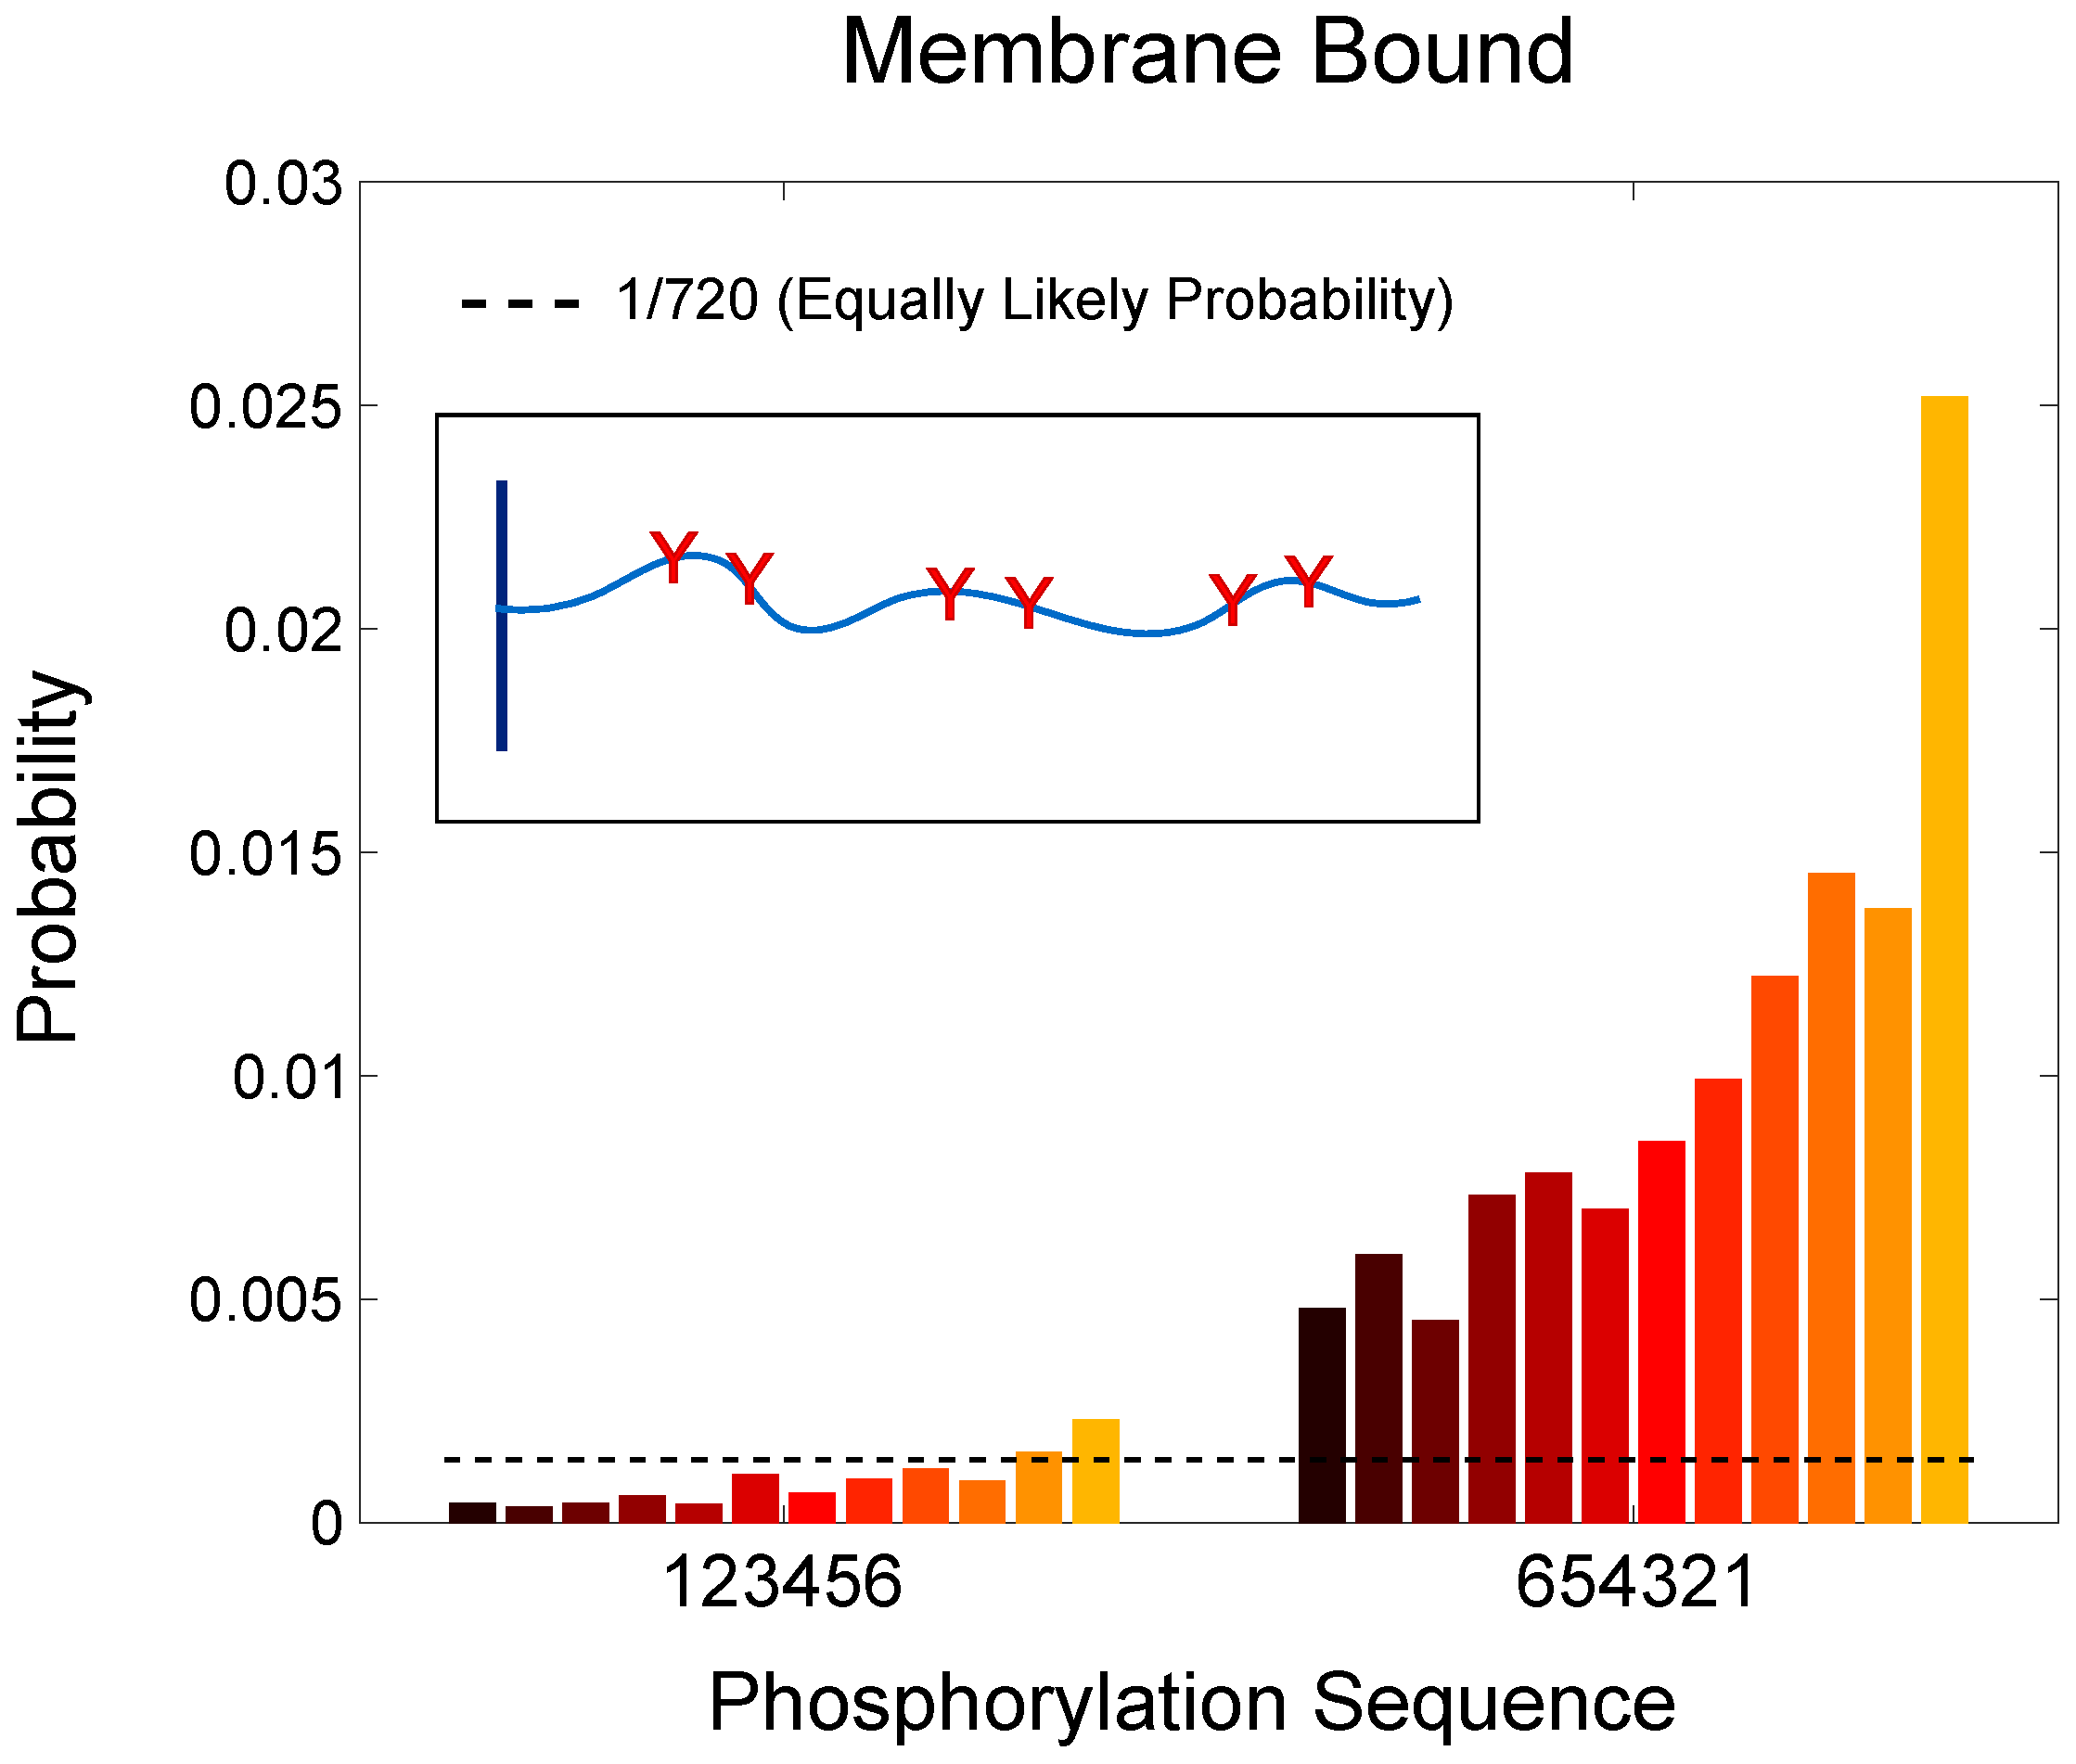
\includegraphics[width=\linewidth]{ResultsFigures/StiffeningSequentialBinding/MemOn/ProbVSSequence.eps}
			\caption{}
		\end{subfigure}
		\begin{subfigure}{0.3\linewidth}
			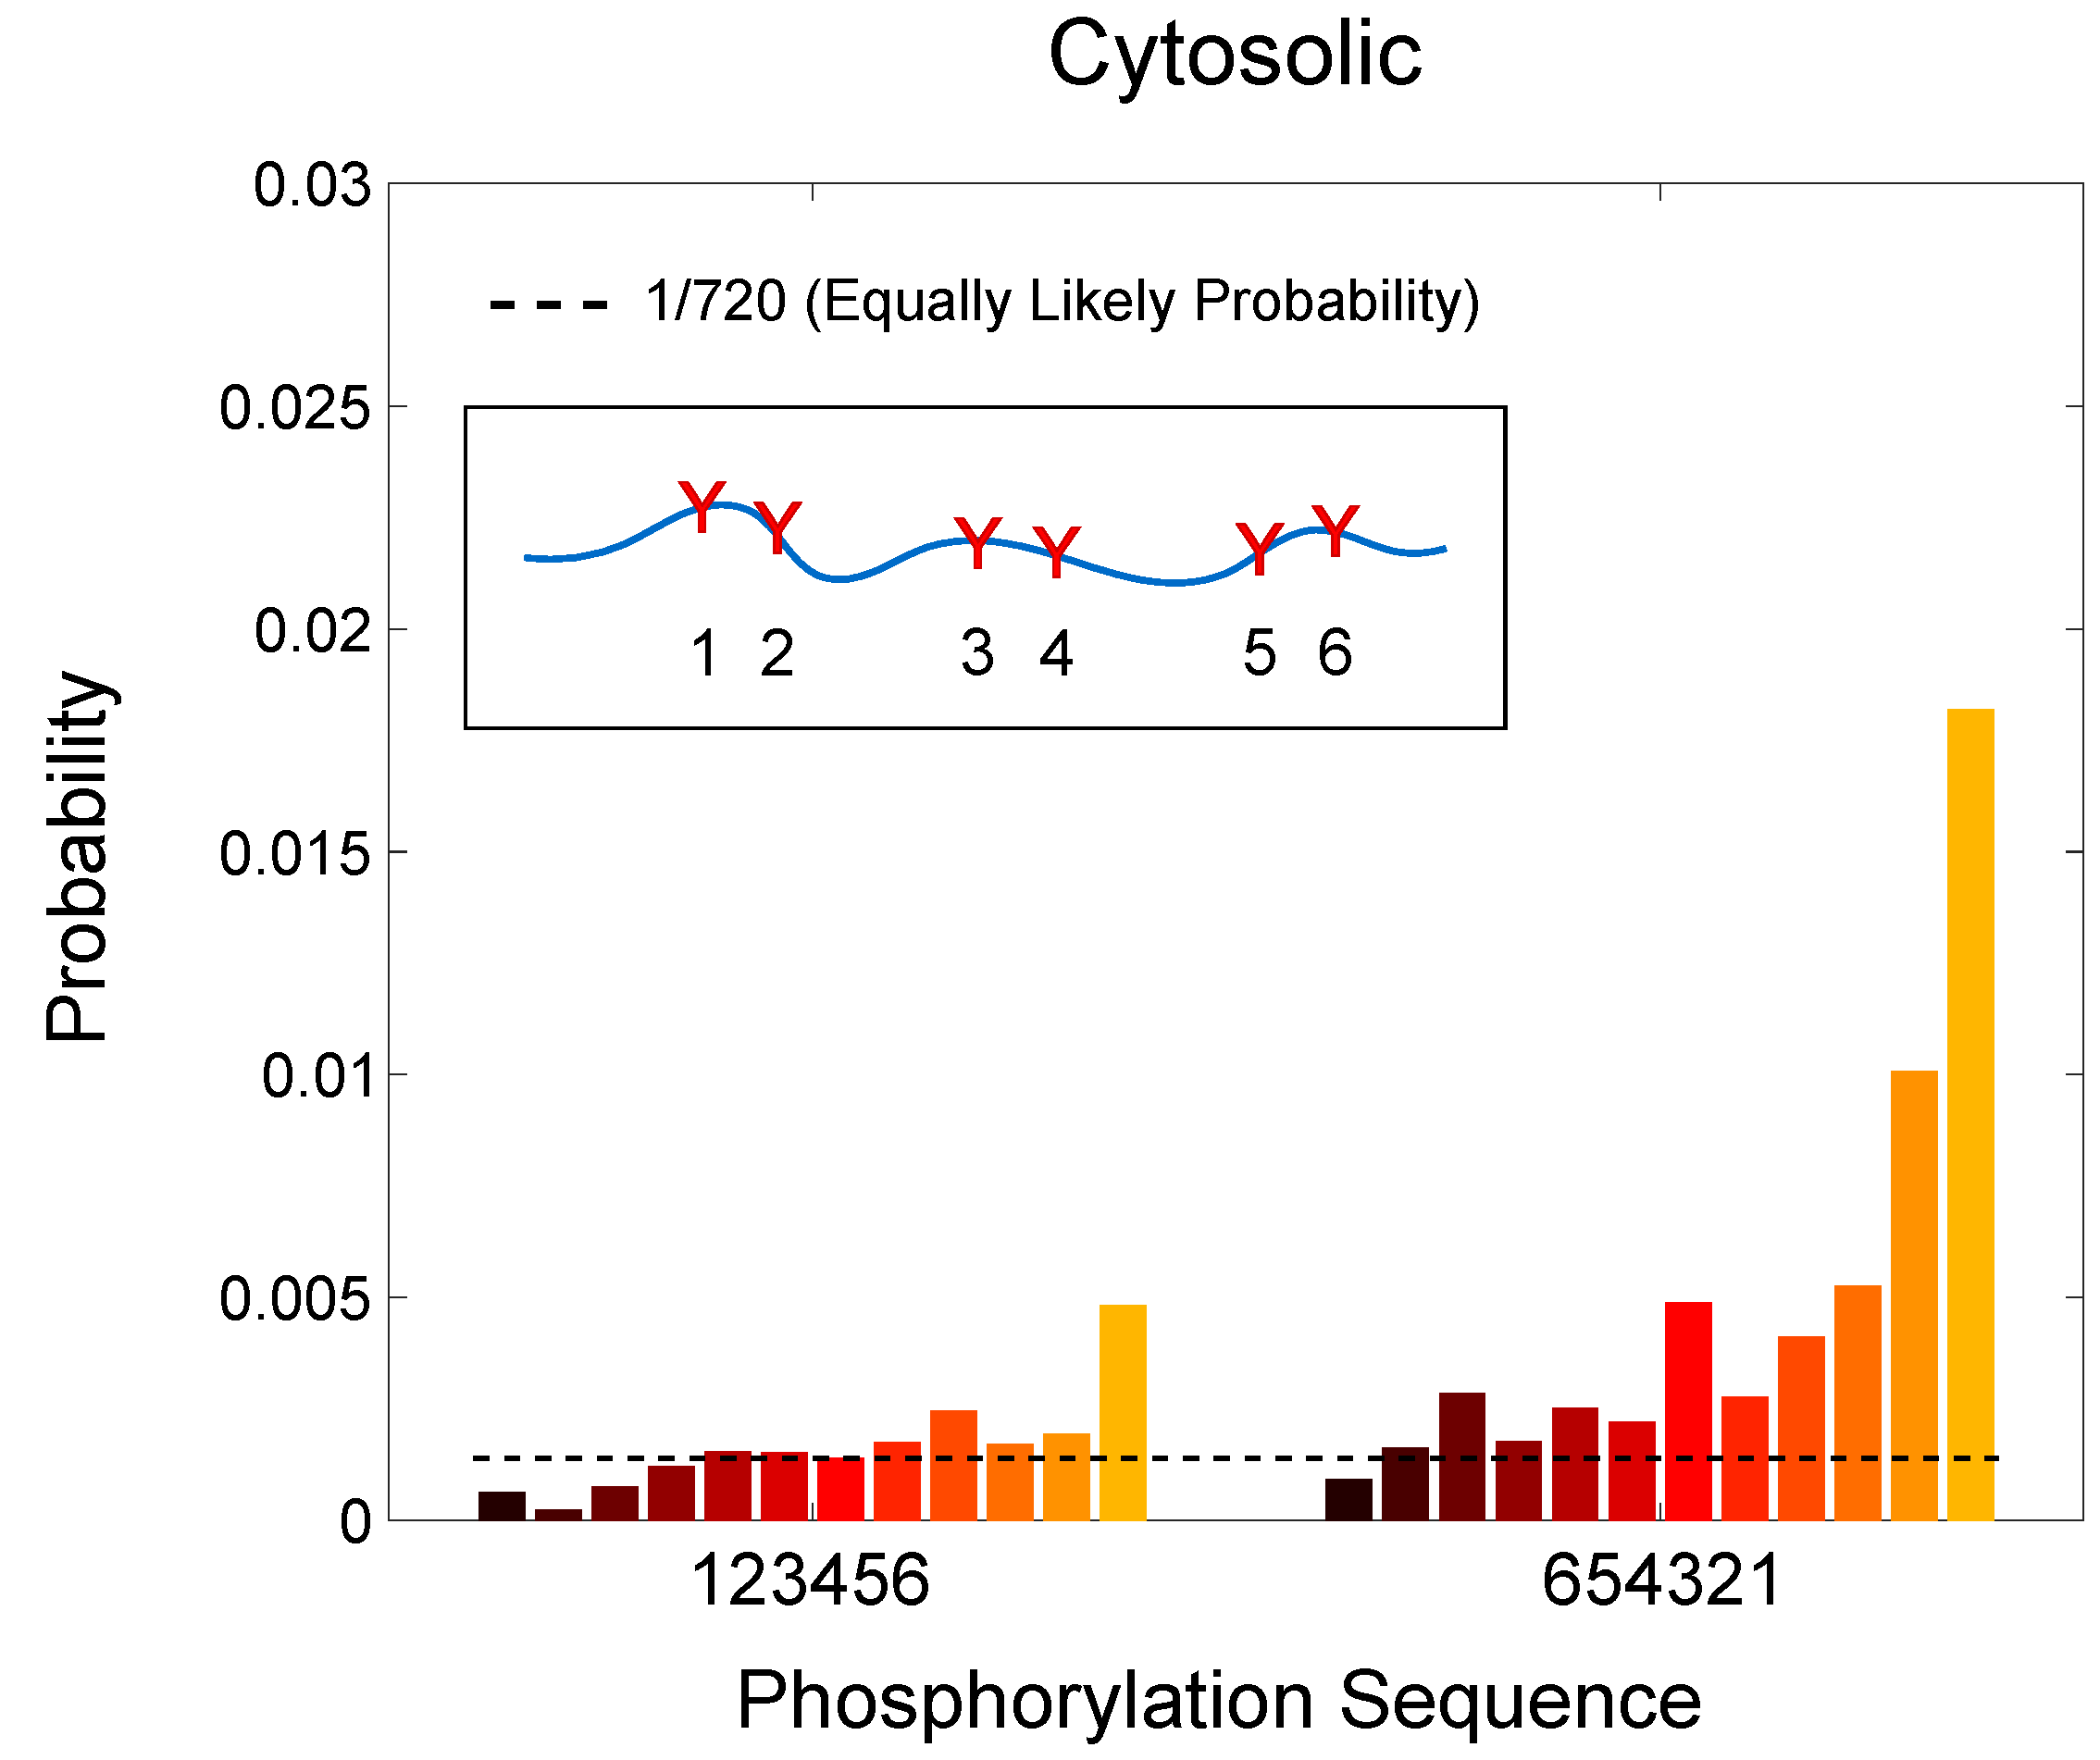
\includegraphics[width=\linewidth]{ResultsFigures/StiffeningSequentialBinding/MemOff/ProbVSSequence.eps}
			\caption{}
		\end{subfigure}
		\begin{subfigure}{0.3\linewidth}
			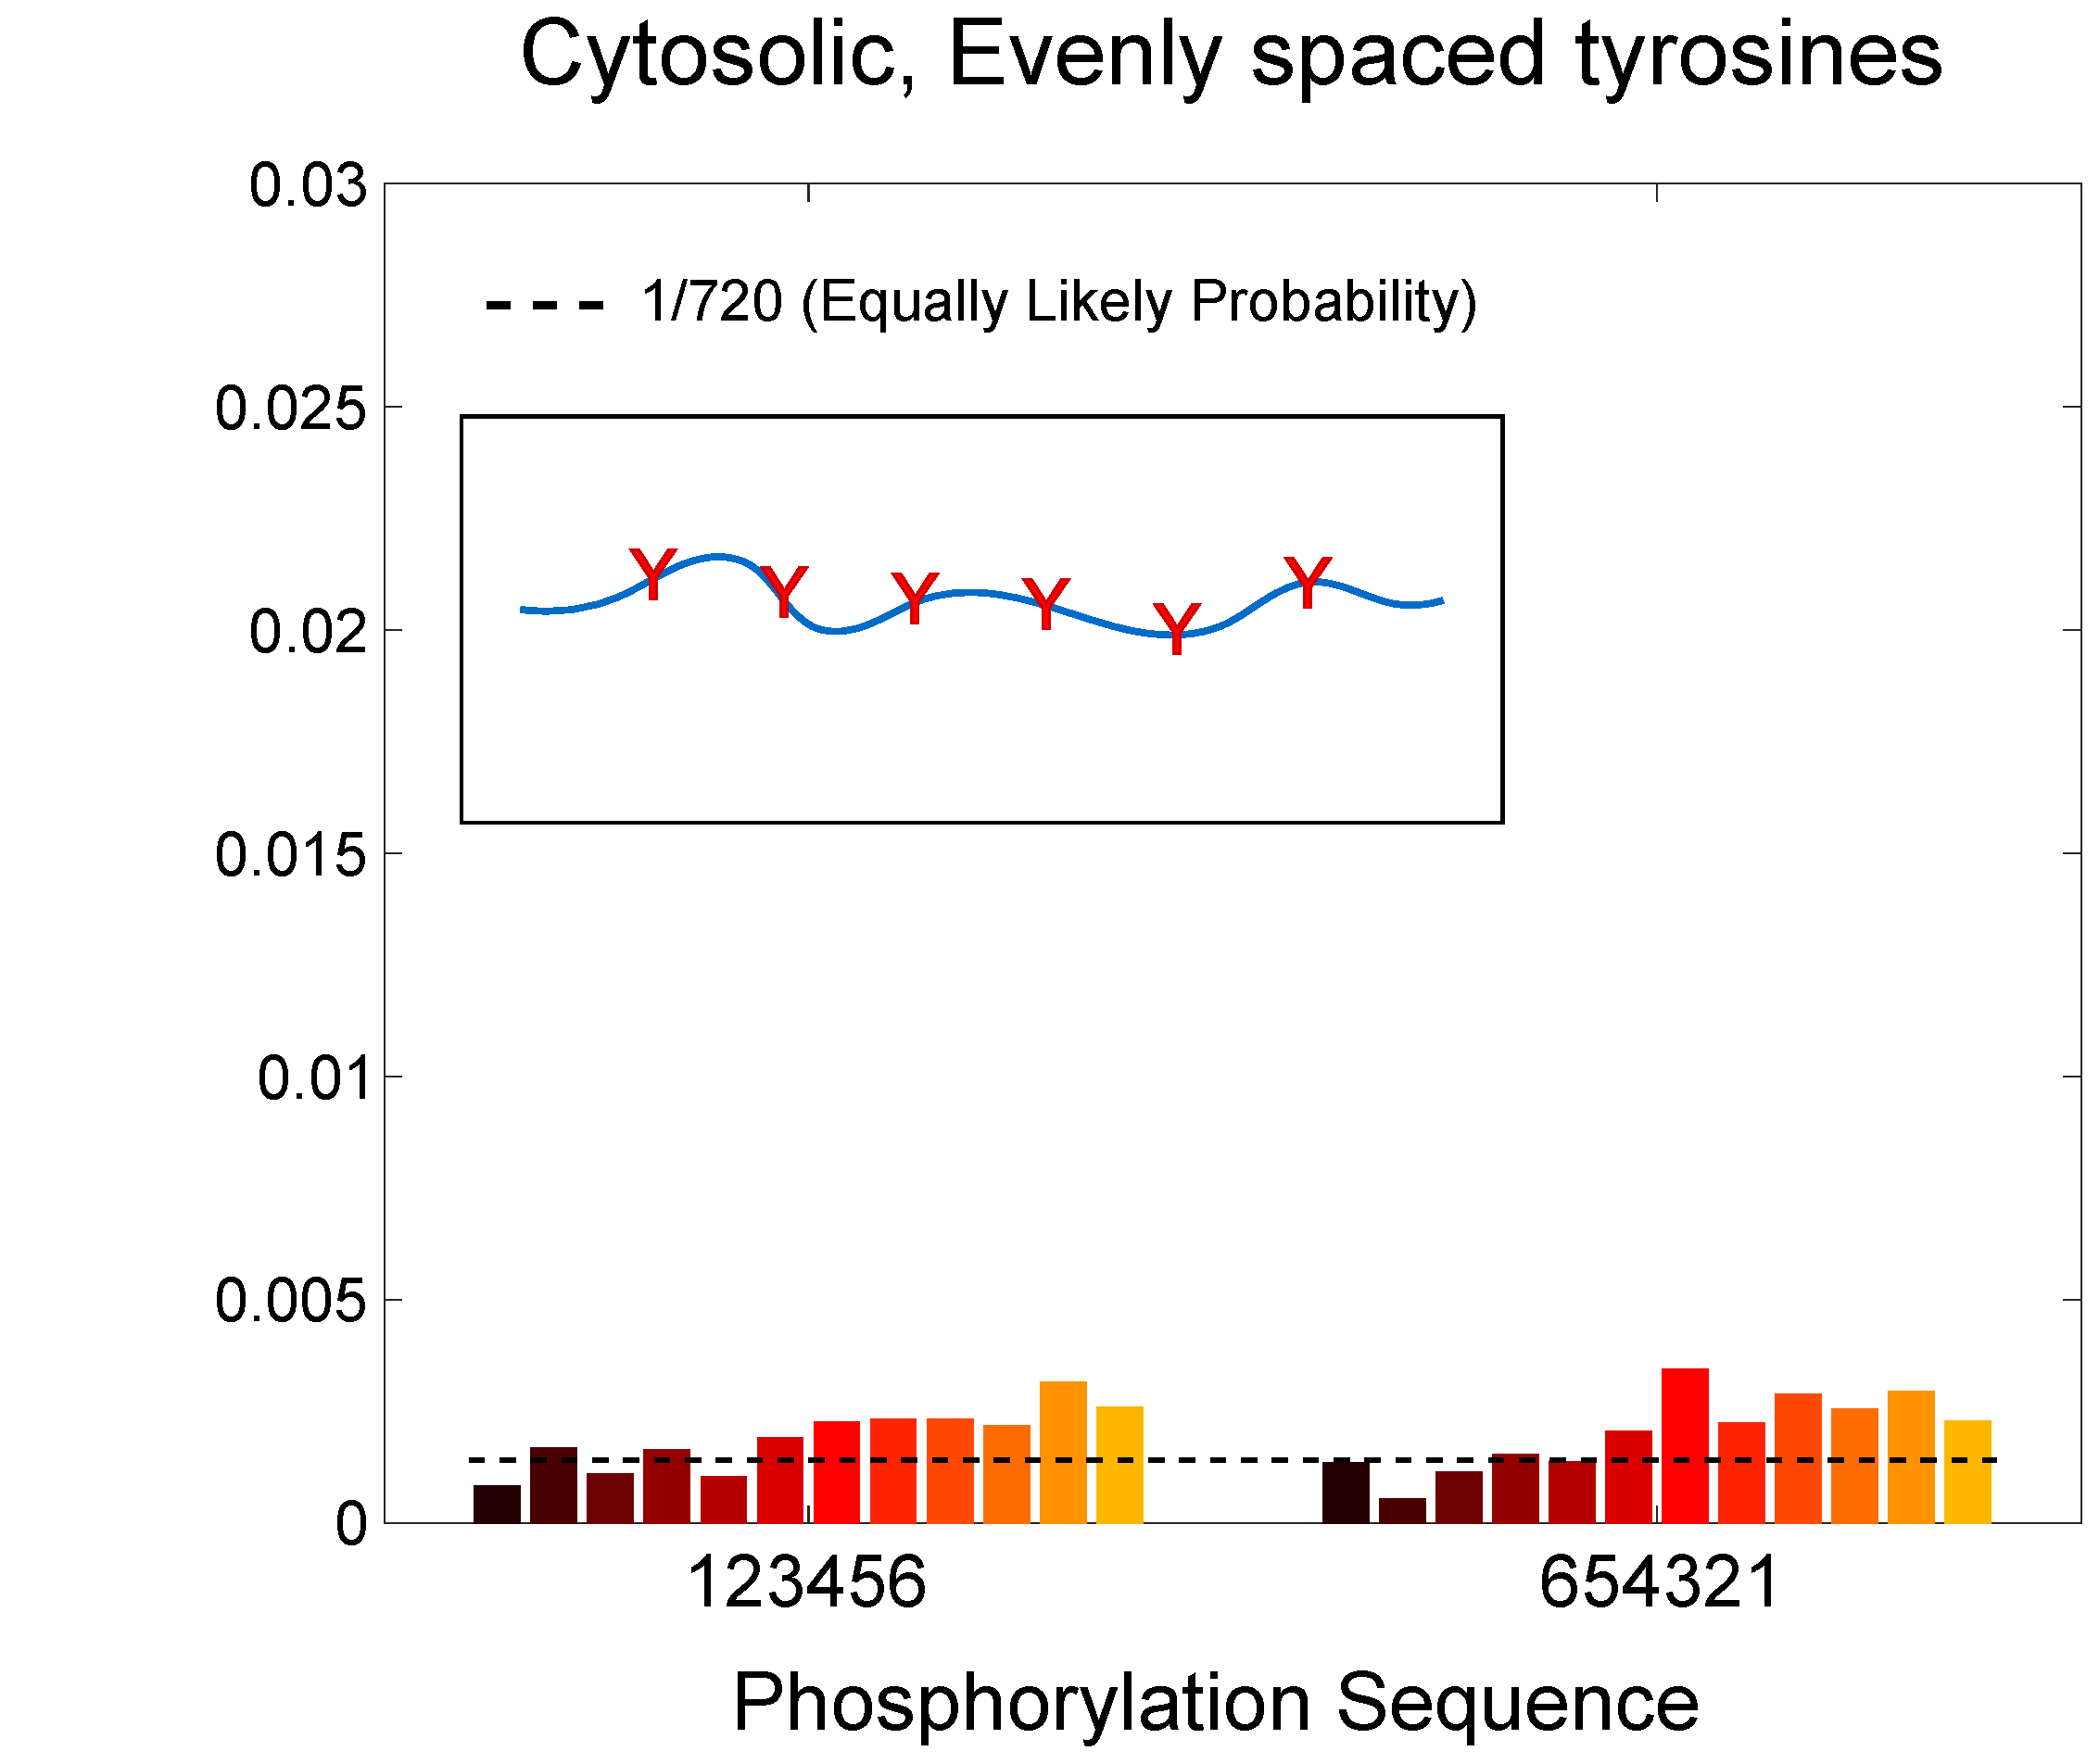
\includegraphics[width=\linewidth]{ResultsFigures/StiffeningSequentialBinding/EvenSites/ProbVSSequence.eps}
			\caption{}
		\end{subfigure}
	\end{center}
	\caption{Probability of phosphorylating membrane proximal to distal (123456) compared with distal to proximal (654321). Equally likely probability of all paths indicated with black, dotted line. (a) CD3$\zeta$ parameters, with membrane. (b) CD3$\zeta$ parameters, without membrane. (c) CD3$\zeta$ length, evenly spaced tyrosine locations, without membrane. \label{fig: StiffeningSeqBind}}
\end{figure}

\subsubsection{Negative cooperativity may arise from local disordering of proteins}

We investigate how dephosphorylation of a locally structured protein would impact future dephosphorylation events. Beginning with a model of CD3$\zeta$ where each tyrosine has been locally structured, we investigate how dephosphorylation and consequently, local unstructuring, influence the rate of subsequent dephosphorylations. We find that as the degree of local de/structuring increases, future dephosphorylations become less likely. For moderate de/structuring, this can create up to a 2-fold negative cooperative effect on the dephosphorylation rates from the first to the sixth event (Fig. \ref{fig: DephosMemOnCoop}).


\begin{figure}[H]
	\begin{center}
		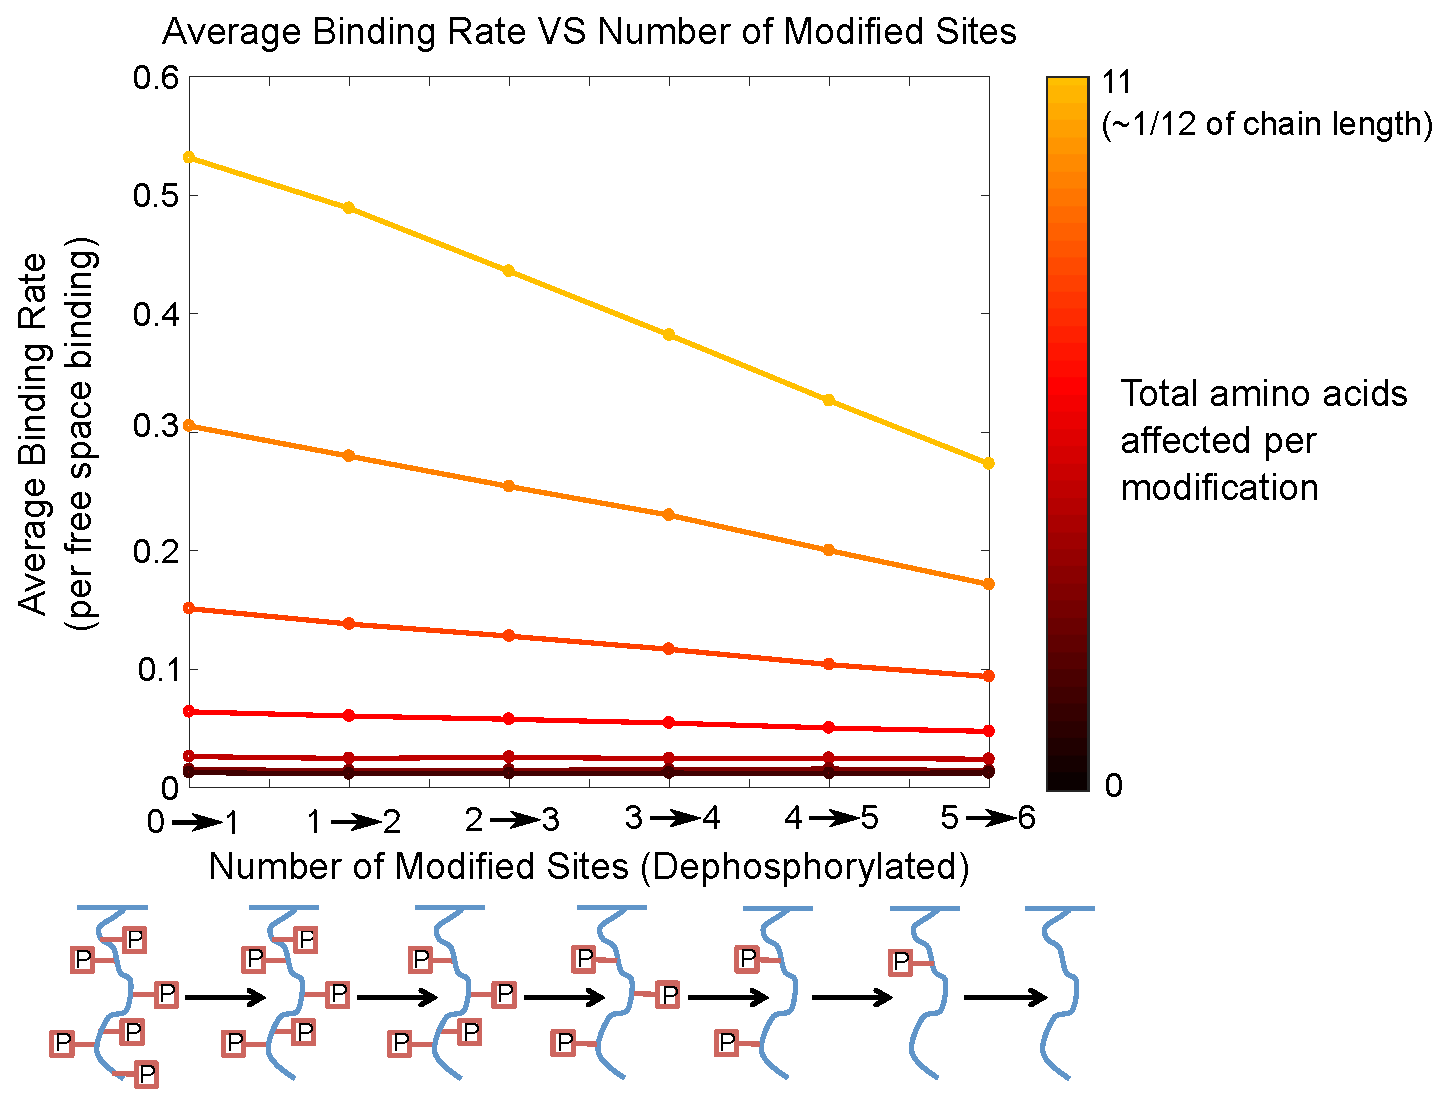
\includegraphics[width=0.8\linewidth]{ResultsFigures/CD3ZetaStiffeningMembraneOn/Dephosphorylation/AvgBindVSTotalModified5.eps}
		\caption{(Above) Simulated average binding rates of Lck to CD3$\zeta$ for different levels of dephosphorylation given a specified degree of local unstructuring (none $\rightarrow$ black, low $\rightarrow$ red, high $\rightarrow$ orange).\label{fig: DephosMemOnCoop}}
	\end{center}
\end{figure}


\subsubsection{Future Work: Quantifying cooperativity from reversible phosphorylation with Hill coefficients}

We will create Hill curves of phosphorylation, dephosphorylation, and reversible phosphorylation. This will allow us to better understand and communicate our results. In particular, the Hill curve of reversible phosphorylation will indicate if ultrasensitivity is achievable through this mechanism. 

\subsubsection{Future Work: Exploring sequence of binding from dephosphorylation and reversible phosphorylation}

We will continue to investigate if phosphorylation, dephosphorylation or reversible phosphorylation naturally impose a sequence of binding. We will introduce a ranking system for the paths in order to do a full analysis of all possible paths. This will help analyze the likelihood of any of the non-sequential paths. Exploring all sequences. will elucidate whether sequential binding occurs when both phosphorylation and dephosphorylation are impacting the polymer simultaneously. 





%%%%%%%%%%%%%%%%%%%%%%%%%%%%%%%%%%%%%%%%%%%%%%%%%%%%%%%%%%%%%%%%%%%%%%%%%%%%%%%%%%%%%%%%%%%%%%%%%%%%%
%%%%%%%%%%%%%%%%%%%%%%%%%%%%%%%%%%%%%%%%%%%%%%%%%%%%%%%%%%%%%%%%%%%%%%%%%%%%%%%%%%%%%%%%%%%%%%%%%%%%%
\subsection{Discussion}

%\hl{What is the definition of cooperativity?  How does this compare to the 'not modifying the switch-like response? vs potency? vs ultrasensitivity?}
%\hl{Question: is this 'cooperativity', how does that influence the network? (refering to local structuring enhancing rate)} 

%%%%
%
%%%%

% matches data, many systems, design principle


% summary of results

% steric occlusion
When binding to disordered proteins, ligands experience significant steric occlusion from their binding sites. We show that this depends on disordered protein length, ligand size, binding site location, and presence of a surface.
% multiple phosphorylation
For disordered proteins with multiple binding sites, disorder leads to global interactions between these sites giving rise to nonlinear effects: positive cooperativity due to disorder-to-order transitions, negative cooperativity from order-to-disorder transitions, and emergent sequential binding. 
This provides a method of achieving nonlinear signaling behavior from a protein with no native structure.	


% rate enhancement of phosphorylation
If we assume the disordered protein undergoes disordered-to-order transitions upon PTM, we find a significant enhancement of the binding rate. 
	% - matches data
	We find that for a simulated TCR CD3$\zeta$ chain, there is an enhancement of phosphorylation rate that can help explain our previously published experimental data \cite{Mukhopadhyay2016}.
	% - many systems
	There are several examples of disordered-to-order transitions upon PTM \cite{He2015, Bah2015, Chin2016}. It is possible these systems could exhibit this same rate enhancement.
	% - design principle
	Positive cooperativity has been extensively studied both theoretically and experimentally \cite{Levantino2012, Monod1965, Jakubik1997, Koshland1966} . It gives rise to many signaling behaviors, including sensitivity to ligand concentration.




% why positive cooperativity is important
%	% 
%We find that phosphorylation-induced local disordered-to-ordered transitions of a disordered protein with multiple phosphorylation sites will enhance the rate of future phosphorylation events. Local disordered-to-ordered transitions are sufficient to create positive cooperativity of PTMs. Positive cooperativity can increase the sensitivity of a response to changes in ligand concentration and increase the potency of signaling responses. This provides one method of achieving nonlinear signaling behavior from a protein with no native structure, assuming high kinase to phosphatase concentration ratio. 
%




% negative cooperativity
Conversely, if we assume a protein undergoes an order-to-disorder transition upon PTM (e.g. dephosphorylation), we find a reduction of the binding rate.
	% - concern of null effects
	If the rate reduction upon disorder (e.g. upon dephosphorylation) were to match the rate enhancement from local structuring (e.g. upon phosphorylation), it is in principle possible to negate the nonlinear behavior displayed above.
	% - results from TCR
	When we simulate dephosphorylation of the TCR CD3$\zeta$ chain, we find only a low reduction of the binding rate compared to the enhancement from phosphorylation.
	% - not strong enough to counter phosphorylation effect
	Therefore, we expect to maintain the nonlinear signaling behavior induced by disordered-to-ordered transitions.
	

%
%% why negative cooperative effects of dephosphorylation matter to the system
%Conversely, if we assume a low kinase to phosphatase ratio, we find that dephosphorylation-induced local unstructuring can create a mild reduction of rates of future dephosphorylations. A negative cooperative dephosphorylation step could bias the system towards phosphorylation, since dephosphorylation events hinder future dephosphorylations, but phosphorylation is positively cooperative. However, it could decrease the average phosphorylation state, since as more tyrosines are phosphorylated, it is easier for both the kinase and phosphatase to bind. 

%\hl{is this rest of the stuff relevant? : This can confer negative cooperativity to the system, endowing signaling systems with two features: high turnover of ligands even in high ligand concentration (which might be advantageous if ligands are involved in other reactions), and constant signaling activity in low ligand concentration. Similarly, this might reduce the impact of inhibitors, requiring much higher concentrations of inhibitor to completely turn off signaling.}
%
%% discussion of hypotheses for reversible phosphorylation based on current results/experimental evidence
%Disordered-to-ordered transitions create these signaling characteristics when kinase and phosphatase concentrations are unbalanced. Future work will examine how the ratio of their concentrations impacts the cooperative effects of the system. However, evidence for positive cooperativity suggests a regime of high kinase to phosphatase post-TCR triggering. This is further supported by evidence of spatial segregation of phosphatase CD148 after TCR triggering. \hl{cite} 

% benefit of sequential phosphorylation
Sequential binding arises even when we assume all binding sites are identical. This phenomenon occurs without disordered-to-ordered transitions. 
	% - location location location
	Part of this sequential preference is due to the locations of the binding sites along the polymer. Even small differences in binding probabilities can lead to large differences in the probability of a particular sequence.
	% - membrane matters
	For membrane bound disordered proteins, part of the emergence of sequential binding is due to high preference to bind (membrane-) distal-to-proximal compared to proximal-to-distal.
	% - design principle
	Sequential binding is another phenomenon which has been extensively theoretically studied (cite cite cite) and has been shown to create nonlinear signaling behavior, such as ultrasensitivity.	
	% - obligate vs preferential
	Note that theoretical studies (cite) focus on `obligate' sequential binding, where each event is required for the next to occur. Our work reveals emergent `preferential' sequential binding, where the sequence is likely to form but not required. How these differ is an interesting question for future study. 
		
%We also find preferential sequential phosphorylation of a membrane-anchored disordered protein occurs naturally. Local structuring is not required for preferential sequential binding, but does enhance the magnitude of the preference. \hl{Does it? Or all the ratios the same?  This seems like an important question.} Sequential binding can create or enhance ultrasensitivity, allowing large changes in response with small changes in signal. \hl{cite Omer?}

% how these results generalize to other systems?
%
%
%
%% conclusion
%Both disordered-to-ordered transitions and membrane-anchoring of disordered proteins can create nonlinear cooperative effects in the signaling network. 



%%%%%%%%%%%%%%%%%%%%%%%%%%%%%%%%%%%%%%%%%%%%%%%%%%%
\end{document}
%%%%%%%%%%%%%%%%%%%%%%%%%%%%%%%%%%%%%%%%%%%%%%%%%%%





